\documentclass{article}
\usepackage{graphicx} % Required for inserting images
\usepackage{setspace}
\usepackage{float}
\usepackage{todonotes}
\usepackage{amsmath}
\usepackage[ngerman]{babel}

\title{researchProject}
\author{Mr Green Pepper}
\date{February 2025}

\begin{document}
\listoftodos
\doublespacing
\maketitle

\tableofcontents

\part{Modell}
\section{Allgemeine Modellerklärung}
\subsection{Variablen und Abkürzungen}
\todo{sauber und ausführlich machen }
Groß geschriebene Variablen werden endogen ermittelt. Klein geschriebene Variablen werden exogen vorgeschrieben.\\

\begin{tabular}{|c|c|}
        $RL$ & Regelleistungsmarkt\\
        $DA$ & Day Ahead Markt \\
        $RA$ & Regelarbeitsmarkt \\
        $r$ & Rate mit der der Stromspeicher geladen/entladen werden kann \\
        $a$ & Anschlusskapazität \\
        $Q^i_{y}$ & Gebotsmenge der Art i(=in/out) am Markt y \\
        ($X^i_{y})$ & (lineare Gebotsmenge der Art i(=in/out) am Markt y) \\
        $P^i_{y}$ & Gebotspreis der Art i(=in/out) am Markt y\\
        $\omega^i_{y}(P^i_{y})$ & Gebotswahrscheinlichkeit für $P^i_{y}$\\
        $p^i_{y}(s^i_y)$ & Gebotspreis der Art i(=in/out) am Markt y für Szenario $s^i_y$\\
        $\omega^i_{y}(s^i_y)$ & Gebotswahrscheinlichkeit für entsprechendes Preisszenario $s^i_y$\\
        $c^i_y$ &  Marktclearingpreis der Art i(=in/out) am Markt y\\
        $B^i_y$ &  Binäre Variable die den Zuschlag (B=1) der Art i(=in/out) am Markt y signalisiert\\
        $M$ &  eine sehr große Zahl\\
    \end{tabular}
\label{tab:my_label}\\
\\

\subsection{Allgemeine Modellerklärung}
Zur Analyse des vorliegenden Problems wird eine stochastische Programmierung verwendet. 
(Zur Vereinfachung werden zuerst alle Formeln für nur einen Zeitschritt aufgestellt. Am Ende wird die Zeitvariable entsprechend hinzugefügt.)
\todo{ausführliche Erklärung stochastische Programmierung}
\\
Das grundlegende Modell stellt einen Energiespeicher da, der am Regelleistungsmarkt, Day Ahead Markt und Regelarbeitsmarkt vermarktet werden kann. Der darraus resultierende Profit soll maximiert werden. Für jede Teilentscheidung/Markt existiert ein eigenes Modell. So kann, für jedes Teilmodell, vermieden werden die anschließenden Marktergebnisse (Zuschlag oder Ablehnung) zu integrieren. Dies ist wichtig, da anderen Falls der Algorithmus allwissend wäre und nur perfekte Gebote errechnen würde. Die Ergebnisse eines jeden Teilmodells werden immer an das nachfolgende Modell übergeben und erst an dieser Stelle ausgewertet. Jedes Teilmodell ermittelt Mengengebote zu bestimmten Preisen. Die verschiedenen Preise werden durch verschiedene Szenarien abgebildet. Jedem Szenario ist eine bestimmte Wahrscheinlichkeit zugeordnet. (Die Preis-Wahrscheinlichkeits-Kombinationen der verschiedenen Szenarien wurden vorher exogen mittels SARIMA-Analyse ermittelt.) Ein Gebot stellt sich dann wie folgt dar:

$Q(s) * p(s) * \omega(s)$\\
Die Daten hierfür lassen sich exemplarisch wie folgt darstellen:\\
\begin{tabular}{c|c|c}
     Szenario $s$& Preis $p(s)$ & Wahrscheinlichkeit $\omega(s)$ \\
     s1       & 90 & 0.6 \\
     s2       & 100 & 0.5 \\
     s3       & 110 & 0.4 \\
\end{tabular}\\


Dabei repräsentiert die Wahrscheinlichkeit die Chance für einen Zuschlag zum zugeordneten Szenariopreis. Ein Zuschlag bei gegebenem Gebot wird als eintreffen des Szenarios interpretiert. Ein geringerer Gebotspreis führt immer zu einer höheren Zuschlagswahrscheinlichkeit. Die Summe aus der Chance für einen Zuschlag und der Chance für eine Ablehnung ergibt dabei immer 1. Die Äste des Szenariobaums stellen dabei die Unterschiedlichen Preisoptionen dar. Mit einem Mengengebot auf einen bestimmten Preis "aktivieren" wird der entsprechende Teil des Szenariobaums aktiviert. Da die gesamte Menge durch $\sum_s Q(s) \leq r$  restriktiert ist, kann eine einzelne Menge (z.B.: 1 MW) nur einmal vergeben werden. Theoretisch ist es möglich, dass unterschiedliche Mengengebote zu unterschiedlichen Preisszenarien erfolgen. Praktisch errechnet der Algorithmus welcher Ast des Szenariobaums den höchsten Erwartungswert ($w(s)*p(s)$) besitzt und bietet entsprechend die maximale Menge an dieser Stelle. \\
 
Im ersten Schritt wird die optimale Entscheidung am Regelleistungsmarkt berechnet. Hierfür werden die Erwartungswerte aller möglichen Szenarien ausgerechnet (siehe 1.4).\\

Im zweiten Schritt werden die, vorher errechneten, Ergebnisse (Mengengebote zum entsprechenden Preis) als exogene Parameter in das 2. Modell eingefügt. Es folgt eine Auswertung ob zum entsprechenden Gebot ein Zuschlag erfolgt. Anschließend wird, wie im vorherigen Schritt, die optimale Entscheidung für den Day Ahead Markt bestimmt (siehe 1.4.2).\\

Im letzten Schritt werden die Ergebnisse des Day Ahead Marktes in das 3. Modell integriert. Nachfolgend wird überprüft ob zum entsprechenden Gebot ein Zuschlag erfolgt. Zum Schluss wird die optimale Entscheidung am Regelarbeitsmarkt ermittelt (siehe 1.4.3).\\
\\





\subsubsection{Preisvorhersage}
Die verschiedenen Preis Szenarien werden mittels SARIMA Analyse exogen errechnet. Die SARIMA Analyse errechnet eine Wahrscheinlichkeitsverteilung (mehr dazu im Abschnitt Preisvorhersage), welche zu jedem Preis dessen Eintrittswahrscheinlichkeit angibt. Zu Vereinfachungszwecken werden die kontinuierlichen Preis-Wahrscheinlichkeits-Pärchen per Szenario Reduktion [N. Growe-Kuska, H. Heitsch, and W. Romisch, “Scenario reduction and scenario tree construction for power management problems,” in Proc.
2003 IEEE Bologna Power Tech Conf., vol. 3, Jun. 2003, pp. 7.] auf signifikante Szenarion reduziert.
Diese diskreten Preis-Wahrscheinlichkeits-Pärchen werden mathematisch über einen Parameter/Binär-Variablen Kombination abgebildet.\\
\\
\textbf{Beispiel: Umwandlung kontinuierliche Variable zu Diskreter:}
\\
Betrachtet werden folgende diskrete Preis-Wahrscheinlichkeits-Pärchen aus einer beispielhaften Szenarioreduktion:\\
\\
\begin{tabular}{c|c|c}
     Szenario $s_{DA}$& Preis $p_{DA}(s_{DA})$ & Wahrscheinlichkeit $\omega_{DA}(s_{DA})$ \\
     s1       & 90 & 0.6 \\
     s2       & 100 & 0.5 \\
     s3       & 110 & 0.4 \\
\end{tabular}\\
\\

$P_{DA} * \omega_{DA}(P_{DA}) \rightarrow \sum_{s_{DA}} p_{DA}(s_{DA}) * \omega_{DA}(s_{DA})$\\

\todo{Erklärung mit summe wahrscheinlichkeiten 1}

 Hier und im folgenden weggelassen ist jeweils die Gegenwahrscheinlichkeit $1-\omega_{DA}(s_{DA})$ da sie die Ablehnung des Gebots repräsentiert und somit in der Ertragsrechnung mit 0 multipliziert werden würde und entsprechend entfällt.\\
\\

\subsection{Marktmodelle}

Das Modell ist in der Lage an drei Märkten zu bieten. Ein Gebot umfasst immer eine Menge sowie einen dazu gehörigen Preis. Zuerst erfolgt das Gebot am Regelleistungsmarkt, dann am Day Ahead Markt und schließlich das Gebot am Regelarbeitsmarkt.
\todo{Übersicht über zeitlichen Ablauf der einzelnen Märkte}

Dabei ergibt sich der zu maximierende Ertrag wie folgt:

$Ertrag = Menge * Preis$

In der stochastischen Programmierung wird eine Wahrscheinlichkeit hinzugefügt welche angibt wie wahrscheinlich der Zuschlag zum entsprechend gebotenen Preis ist.\\

$Ertrag = Menge * Preis * Wahr(Preis)$\\

In den folgenden Kapiteln werden zuerst die einzelnen Märkte  individuell beschrieben. (siehe 1.3.1 bis 1.3.3).
Nachfolgend wird die Überführung der Einzelmarktprobleme in eine Gesamtentscheidung erläutert.
1.4 skizziert hierfür zuerst die schematische Berechnung der Einzelentscheidungen.
1.4.1 bis 1.4.3 erläutern dann die detaillierten Einzelberechnungen.

\subsubsection{Regelleistungsmarkt}
Für den Regelleistungsmarkt ergibt sich dann die folgende Zielfunktion.\\

$max Profit_{RL} = Q_{RL} * p_{RL} * \omega_{RL}(p_{RL})$

Durch einsetzen der vorhergesagten Preise ergibt sich dann die folgende Gleichung:\\

$max Profit_{RL} = \sum_{s_{RL}} Q_{RL}(s_{RL}) * p_{RL}(s_{RL}) * \omega_{RL}(s_{RL})$\\

Zu beachten ist, dass auch die Menge nun Szenarioabhängig ist, so kann theoretisch auf für jedes angenommene Szenario separat geboten werden. Praktisch ist dies nicht an zu nehmen, da der Algorithmus die höchst mögliche Menge immer dem höchsten Preiserwartungswert wahrscheinlich zuordnen wird. Auf diese Weise dient die Menge als abstrakte binäre Aktivierungsvariable der verschiedenen Preisszenarien.
\todo{den Part Menge als abstrakte binäre Aktivierungsvariable eventuell nochmal überarbeiten und entsprechend oben anpassen }
\todo{eventuell binär variable nur an Preis koppeln und das dann anders heraus ziehen}
Für die anschließenden Märkte ist es wichtig zu wissen ob das Gebot angenommen wurde oder nicht. Dies wird über eine binäre Variable $B_{RL}$ repräsentiert.

$max Profit_{RL} = \sum_{s_{RL}} Q_{RL}(s_{RL}) * B_{RL}(s_{RL}) * p_{RL}{RL}(s_{RL}) * \omega_{RL}(s_{RL})$\\
s.t.:\\
$c_{RL} \leq p_{RL}(s_{RL}) + M * B_{RL}(s_{RL}) $\\
$c_{RL} \geq p_{RL}(s_{RL}) - M * (1 - B_{RL}(s_{RL})) $\\
$B_{RL} \in \{0,1\}$\\
$M$ ist hierbei eine sehr große Zahl. Über die Kombination beider Nebenbedingungen wird sicher gestellt, dass der Lösungsalgorithmus die binäre Variable immer so setzt, dass sie dem tatsächlichen Marktresultat entspricht. So entspricht $B_{RL} = 1$ einem angenommenen Gebot und $B_{RL} = 0$ entspricht einem abgelehnten Gebot.\\
\todo{ausführliche Erklärung zusammenspiel Nebenbedingungen und binär Variable}
\todo{Zitat einfügen}




\todo{Zitat einfügen}
Zu beachten ist das sowohl positive als auch negative Leistungsgebote abgegeben werden können. Die vollständige Zielfunktion drückt sich dann wie folgt aus:\\

\begin{center}
$max_{Q^{in}_{RL}(s_{RL}), Q^{out}_{RL}(s_{RL})} Profit_{RL}$\\ 
$=$\\
$\sum_{s^{in}_{RL}} Q^{in}_{RL}(s_{RL}) * p(s^{in}_{RL}) * \omega_{RL}(s^{in}_{RL}) +$\\
$\sum_{s^{out}_{RL}} Q^{out}_{RL}(s_{RL}) * p(s^{out}_{RL}) * \omega_{RL}(s^{out}_{RL})$\\
\end{center}


(grundlegende Beschränkungen der Definitionsbereiche:)\\
$B^{in}_{RL}(s^{in}_{RL}),B^{out}_{RL}(s^{out}_{RL}) \in \{0,1\}\quad\forall s^{in}_{RL},s^{out}_{RL} $\\
$Q^{in}_{RL}(s^{in}_{RL}),Q^{out}_{RL}(s^{out}_{RL}) \geq 0\quad\forall  s^{in}_{RL},s^{out}_{RL} $\\
(wird später durch Nebenbedingungen des Regelarbeitsmarktes ersetzt:)\\
$\sum_{s^{in}_{RL}}Q^{in}_{RL}(s^{in}_{RL}),\sum_{s^{out}_{RL}}Q^{out}_{RL}(s^{out}_{RL}) \leq r $\\
$a + \sum_{s^{in}_{RL}}Q^{in}_{RL}(s^{in}_{RL})\geq \sum_{s^{out}_{RL}}Q^{out}_{RL}(s^{out}_{RL}) $\\
\todo{alle gleichungen checken wegen $\forall$}
\todo{alle gleichungen mit nummerierung und beschreibung{?} überarbeiten}

\subsubsection{Day Ahead Markt}
Simultan zu dem vorherigen Kapitel ergeben sich dann dich Gleichungen für den Day Ahead Markt.
Der Day Ahead Markt ist der Markt an dem der Strom des Windparks vermarktet wird. Dementsprechend gibt es keine positiven und negativen Gebote.

\begin{center}
$max_{Q_{DA}(s_{DA})} Profit_{DA}$\\ 
$=$\\
$\sum_{s_{DA}} Q_{DA}(s_{DA}) * p(s_{DA}) * \omega_{DA}(s_{DA})$\\

\end{center}
s.t.:\\

s.t.:\\
(grundlegende Beschränkungen der Definitionsbereiche:)\\
$Q_{DA}(s_{DA}) \geq 0\quad\forall  s_{DA} $\\
(wird später durch Nebenbedingungen des Regelarbeitsmarktes ersetzt:)\\

$ \sum_{s_{DA}}Q_{DA}(s_{DA}) \leq r $\\
$a \geq \sum_{s_{DA}}Q_{DA}(s_{DA}) $\\
\todo{annahme perfekte Vorraussicht Windpark}


\subsubsection{Regelarbeitsmarkt}
Simultan zum Regelleistungsmarkt ergibt sich der Regelarbeitsmarkt:
\todo{erklärung zusammenhang regelleistungsmarkt regelarbeitsmarkt}
\begin{center}
	$max_{Q^{in}_{RA}(s_{RA}), Q^{out}_{RA}(s_{RA})} Profit_{RA}$\\ 
	$=$\\
	$\sum_{s^{in}_{RA}} Q^{in}_{RA}(s_{RA}) * p(s^{in}_{RA}) * \omega_{RA}(s^{in}_{RA}) +$\\
	$\sum_{s^{out}_{RA}} Q^{out}_{RA}(s_{RA}) * p(s^{out}_{RA}) * \omega_{RA}(s^{out}_{RA})$\\
\end{center}
s.t.:\\
	(grundlegende Beschränkungen der Definitionsbereiche:)\\
	$Q^{in}_{RA}(s^{in}_{RA}),Q^{out}_{RA}(s^{out}_{RA}) \geq 0 \quad\forall s^{in}_{RA},s^{out}_{RA} $\\
	$Q^{in}_{RA}(s^{in}_{RA}),Q^{out}_{RA}(s^{out}_{RA}) \geq 0\quad\forall  s^{in}_{RA},s^{out}_{RA} $\\


\subsection{Berechnung optimale Einzelentscheidungen}
Um die optimale Erststufenentscheidung zu berechnen wird der Erwartungswert sämtlicher Zweige des Szenario-Baum ausgerechnet.
Die Entscheidung zu welchem Preis am positiven sowie negativen Regelleistungsmarkt geboten werden soll erfolgt zeitgleich.
Daraus ergeben sich 4 Szenarien:
\begin{enumerate}
    \item $RL^{in}$ \& $RL^{out}$ angenommen
    \item nur $RL^{in}$ angenommen
    \item nur $RL^{out}$ angenommen
    \item $RL^{in}$ \& $RL^{out}$ abgelehnt
\end{enumerate}
Es folgt eine systematische Darstellung dieser Rechnung:

    \begin{tabular}{|c|c|}
     \hline
     Formelzeichen & Erklärung \\
      \hline
        $\omega()$ & Wahrscheinlichkeit für Preis/Mengen Kombination \\
       $E()$  &  Ertrag von Preis/Mengen \\
        &   Kombination am Markt \\
       $RL^{in/out}$  &Preis/Mengen Kombination am Regelleistungsmarkt\\ 
       $DA$  & Preis/Mengen Kombination am Day Ahead Markt\\ 
       $RA^{in/out}$  & Preis/Mengen Kombination am Regelarbeitsmarkt\\
        \hline
    \end{tabular}
    \caption{}
    \label{tab:my_label}

\begin{alignat*}{3}
max Profit = \\
\sum \sum \omega(RL^{in})* \omega(RL^{out}) &* \Biggl[E(RL^{in}) + E(RL^{out}) \\
& +\sum_{DA} \omega(DA) *&&\Biggl(E(DA)\\
	&    &&+ \sum_{RA^{in}} \omega(RA^{in}) * E(RA^{in})\\
	&    &&+ \sum_{RA^{out}} \omega(RA^{out}) * E(RA^{out})\Biggr)\\
& +\sum_{DA} (1- \omega(DA) * &&\Biggl(\sum_{RA^{in}} \omega(RA^{in}) * E(RA^{in}) \\
	&    &&+ \sum_{RA^{out}} \omega(RA^{out}) * E(RA^{out})\Biggr) \Biggr]\\
+\sum \sum (1-\omega(RL^{in})) * \omega(RL^{out}) &* \Biggl[E(RL^{in}) + E(RL^{out}) \\
& +\sum_{DA} \omega(DA) *&&\Biggl(E(DA)\\
	&    &&+ \sum_{RA^{in}} \omega(RA^{in}) * E(RA^{in})\\
	&    &&+ \sum_{RA^{out}} \omega(RA^{out}) * E(RA^{out})\Biggr)\\
& +\sum_{DA} (1- \omega(DA)) * &&\Biggl(\sum_{RA^{in}} \omega(RA^{in}) * E(RA^{in}) \\
	&    &&+ \sum_{RA^{out}} \omega(RA^{out}) * E(RA^{out})\Biggr) \Biggr]\\
\end{alignat*}
\begin{alignat*}{3}
+\sum \sum \omega(RL^{in})* (1-\omega(RL^{out}))& * \Biggl[E(RL^{in}) + E(RL^{out}) \\
& +\sum_{DA} \omega(DA) *&&\Biggl(E(DA)\\
	&    &&+ \sum_{RA^{in}} \omega(RA^{in}) * E(RA^{in})\\
	&    &&+ \sum_{RA^{out}} \omega(RA^{out}) * E(RA^{out})\Biggr)\\
 & +\sum_{DA} (1- \omega(DA)) * &&\Biggl(\sum_{RA^{in}} \omega(RA^{in}) * E(RA^{in}) \\
	&    &&+ \sum_{RA^{out}} \omega(RA^{out}) * E(RA^{out})\Biggr) \Biggr]\\
+\sum \sum (1-(\omega(RL^{in})* \omega(RL^{out}))& * \Biggl[E(RL^{in}) + E(RL^{out}) \\
& +\sum_{DA} \omega(DA) *&&\Biggl(E(DA)\\
	&    &&+ \sum_{RA^{in}} \omega(RA^{in}) * E(RA^{in})\\
	&    &&+ \sum_{RA^{out}} \omega(RA^{out}) * E(RA^{out})\Biggr)\\
& +\sum_{DA} (1- \omega(DA)) * &&\Biggl(\sum_{RA^{in}}\omega(RA^{in}) * E(RA^{in}) \\
	&    &&+ \sum_{RA^{out}} \omega (RA^{out}) * E(RA^{out})\Biggr) \Biggr]\\
\end{alignat*}

\subsubsection{Berechnung optimale Erststufenentscheidungen}

Da die einzelnen Mengen, je nach Szenario, unterschiedlichen Restriktionen unterliegen werden ihnen separate Variablen zugewiesen.
Es folgt eine ausführliche Formel für die Berechnung der optimalen Erststufenentscheidung:
(Die einzelnen Mengen Formelzeichen setzen sich wie folgt zusammen:
\begin{enumerate}
    \item $Q$ - Menge
    \item $Q_{\pmb{y}}$ - am welchem Markt die Menge Geboten wird
    \item $Q^{\pmb{i}}_{y}$ - (nur für die Regelmärkte) welche Art von Leistung geboten wird: negativ$\rightarrow$in / positiv$\rightarrow$out
    \item $Q^{i\pmb{r...}}_{y}$ - welchen Restriktionen die Menge unterliegt, da in vorhergehenden Märkten entsprechende Zuschläge erfolgt sind
\end{enumerate}
Beispiele: 
\begin{itemize}
    \item $Q^{outrRL}_{RA}$ - positive Menge am Regelarbeitsmarkt restriktiert durch ein bezuschlagtes Regelleistungsmarkt-Gebot
    \item $Q^{rRL}_{DA}$ - Menge am Day Ahead Markt restriktiert durch ein bezuschlagtes Regelleistungsmarkt-Gebot
    \item $Q^{in}_{RA}$ - negative Menge am Regelarbeitsmarkt mit keinen Restriktionen 
\end{itemize}


\begin{alignat*}{3}  
max Profit  =&\\
for\quad accepted\quad RL\quad in \& out:&\\
\sum_{s^{out}_{RL}}\sum_{s^{in}_{RL}} (\omega_{RL}(s^{in}_{RL})*\omega_{RL}(s^{out}_{RL}))&*\Biggl[Q^{in}_{RL} (s^{in}_{RL}) *p(s^{in}_{RL}) && + Q^{out}_{RL}(s^{out}_{RL}) * p(s^{out}_{RL})\\
		&+ \sum_{s_{DA}}\omega_{DA}(s_{DA})&& * \Biggl(Q^{rRL}_{DA}(s_{DA}) * p(s_{DA}) \\
		&	&& + \sum_{s^{in}_{RA}} Q^{inrRLDA}_{RA}(s^{in}_{RA}) * p(s^{in}_{RA}) * \omega_{RA}(s^{in}_{RA})\\
	&		&& + \sum_{s^{out}_{RA}} Q^{outrRLDA}_{RA}(s^{out}_{RA}) * p(s^{out}_{RA}) * \omega_{RA}(s^{out}_{RA})\Biggr)\\
		& + \sum_{s_{DA}}(1-\omega_{DA}(s_{DA}))&& * \Biggl(\sum_{s^{in}_{RA}} Q^{inrRL}_{RA}(s^{in}_{RA}) * p(s^{in}_{RA}) *             \omega_{RA}(s^{in}_{RA})\\
	&		&& + \sum_{s^{out}_{RA}} Q^{outrRL}_{RA}(s^{out}_{RA}) * p(s^{out}_{RA}) * \omega_{RA}(s^{out}_{RA}) \Biggr) \Biggr]\\
\end{alignat*}
for accepted RL in 	\& declined out:\\
\begin{alignat*}{3}  
+\sum_{s^{out}_{RL}}\sum_{s^{in}_{RL}} (\omega_{RL}(s^{in}_{RL})*(1-\omega_{RL}(s^{out}_{RL})) *&\Biggl[Q^{in}_{RL}(s^{in}_{RL}) * p(s^{in}_{RL})&&\\
		& + \sum_{s_{DA}}\omega_{DA}(s_{DA}) * &&\Biggl(Q^{rRL}_{DA}(s_{DA}) * p(s_{DA}) \\
	&		&& + \sum_{s^{in}_{RA}} Q^{inrRLDA}_{RA}(s^{in}_{RA}) * p(s^{in}_{RA}) * \omega_{RA}(s^{in}_{RA})\\
	&		&& + \sum_{s^{out}_{RA}} Q^{outrDA}_{RA}(s^{out}_{RA}) * p(s^{out}_{RA}) * \omega_{RA}(s^{out}_{RA})\Biggr)\\
		& + \sum_{s_{DA}}(1-\omega_{DA}(s_{DA}))&& \\
	&		&& * \Biggl( \sum_{s^{in}_{RA}} Q^{inrRL}_{RA}(s^{in}_{RA}) * p(s^{in}_{RA}) * \omega_{RA}(s^{in}_{RA})\\
	&		&& + \sum_{s^{out}_{RA}} Q^{out}_{RA}(s^{out}_{RA}) * p(s^{out}_{RA}) * \omega_{RA}(s^{out}_{RA})\Biggr)\Biggr]
\end{alignat*}
for declined RL in\& accepted out:\\
\begin{alignat*}{3}  
\sum_{s^{out}_{RL}}\sum_{s^{in}_{RL}}(1-\omega_{RL}(s^{in}_{RL}))*\omega_{RL}(s^{out}_{RL}))*&\Biggl[Q^{out}_{RL}(s^{out}_{RL}) * p(s^{out}_{RL})&&\\
		& + \sum_{s_{DA}}\omega_{DA}(s_{DA}) && * \Biggl(Q^{rRL}_{DA}(s_{DA}) * p(s_{DA}) \\
	&		&& + \sum_{s^{in}_{RA}} Q^{inrDA}_{RA}(s^{in}_{RA}) * p(s^{in}_{RA}) * \omega_{RA}(s^{in}_{RA})\\
	&		&& + \sum_{s^{out}_{RA}} Q^{outrRLDA}_{RA}(s^{out}_{RA}) * p(s^{out}_{RA}) * \omega_{RA}(s^{out}_{RA})\Biggr)\\
		& + \sum_{s_{DA}}(1-\omega_{DA}(s_{DA}))&& \\
	&		&& * \Biggl(\sum_{s^{in}_{RA}} Q^{in}_{RA}(s^{in}_{RA}) * p(s^{in}_{RA}) * \omega_{RA}(s^{in}_{RA})\\
	&		&& + \sum_{s^{out}_{RA}} Q^{outrRL}_{RA}(s^{out}_{RA}) * p(s^{out}_{RA}) * \omega_{RA}(s^{out}_{RA})\Biggr) \Biggr]
\end{alignat*}
for declined RL in\& out:\\
\begin{alignat*}{3}  
\sum_{s^{out}_{RL}}\sum_{s^{in}_{RL}} (1-(\omega_{RL}(s^{in}_{RL})*\omega_{RL}(s^{out}_{RL})))&*\Biggl[\sum_{s_{DA}}\omega_{DA}(s_{DA}) && *\Biggl(Q_{DA}(s_{DA}) * p(s_{DA}) \\
   	&		&& + \sum_{s^{in}_{RA}} Q^{inrDA}_{RA}(s^{in}_{RA}) * p(s^{in}_{RA}) * \omega_{RA}(s^{in}_{RA})\\
   	&		&& + \sum_{s^{out}_{RA}} Q^{outrDA}_{RA}(s^{out}_{RA}) * p(s^{out}_{RA}) * \omega_{RA}(s^{out}_{RA})\Biggr)\\
		& + \sum_{s_{DA}}(1-\omega_{DA}(s_{DA}))&& \\
	&		&& * \Biggl(\sum_{s^{in}_{RA}} Q^{in}_{RA}(s^{in}_{RA}) * p(s^{in}_{RA}) * \omega_{RA}(s^{in}_{RA})\\
	&		&& + \sum_{s^{out}_{RA}} Q^{out}_{RA}(s^{out}_{RA}) * p(s^{out}_{RA}) * \omega_{RA}(s^{out}_{RA})\Biggr) \Biggr]
\end{alignat*}




\textbf{Nebenbedingungen}\\

Anschlusspunkt:\\
$a + Q^{in}_{RA} \geq Q^{outrRLDA}_{RA} + Q^{rRL}_{DA}$ \\
$a + Q^{in}_{RA} \geq Q^{outrDA}_{RA} + Q_{DA}$ \\
$a + Q^{in}_{RA} \geq Q^{out}_{RA}$ \\
Batterie Restriktionen:\\
$Q^{out}_{RL}, Q^{in}_{RL}, Q_{DA}, Q^{out}_{RA}, Q^{in}_{RA}, Q^{outrRL}_{RA}, Q^{inrRL}_{RA}, Q^{outrDA}_{RA}, Q^{inrDA}_{RA}, Q^{outrRLDA}_{RA}, Q^{inrRLDA}_{RA} \leq r$\\
Markt Restriktionen:\\
$\sum_{s^{out}_{RA}} Q^{outrRL}_{RA} \geq \sum_{s^{out}_{RL}} Q^{out}_{RL} $\\
$\sum_{s^{in}_{RA}} Q^{inrRL}_{RA} \geq \sum_{s^{in}_{RL}} Q^{in}_{RL} $\\
$\sum_{s^{out}_{RA}} Q^{outrRLDA}_{RA} \geq \sum_{s^{out}_{RL}} Q^{out}_{RL} $\\
$\sum_{s^{in}_{RA}} Q^{inrRLDA}_{RA} \geq \sum_{s^{in}_{RL}} Q^{in}_{RL} $\\




\subsubsection{Berechnung optimale Zweitstufenentscheidung}
Die vorher berechneten optimalen Gebotsmengen $q^{in^*}_{RL}$ \& $q^{out^*}_{RL}$ und Preise $p(s^{out}_{RL})$ \& $p(s^{in}_{RL})$  werden nun exogen in das Modell eingespeist. Sie werden mit einer binären Variable gekoppelt welche angibt ob zum entsprechenden Preis ein Zuschlag erfolgt. Die korrekte Setzung der binären Variable wird über eine Kombination aus 2 Nebenbedingungen sicher gestellt.\\
Schematisch stellt sich dies dann wie folgt dar:\\
$\sum_s q^*(s) * p(s) * B(s)$\\
s.t.:\\
$c \leq p(s) + M * B(s)\quad\forall s $ \\
$c \geq p(s) - M * (1 - B(s))\quad\forall s $ \\

\begin{tabular}{c|c}
    $c$ & Clearing Preis Markt \\
    $p(s)$ &  Gebotspreis für Szenario s \\
    $M$ & sehr große Zahl\\
    $B(s)$ & binäre Variable welche angibt ob Szenariopreis zuschlag erhalten hat\\
\end{tabular}\\

Das gesamte Modell für den Day Ahead Markt ergibt sich dann wie folgt dar:
\begin{alignat*}{3}  
max Profit  =&\\
q^{in^*}_{RL} (s^{in}_{RL})& * p(s^{in}_{RL}) * B^{in}_{RL} (s_{RL}) \\
+ q^{out^*}_{RL}(s^{out}_{RL})& * p(s^{out}_{RL}) * B^{out}_{RL} (s_{RL})\\
		&+ \sum_{s_{DA}}\omega_{DA}(s_{DA})&& * \Biggl(Q_{DA}(s_{DA}) * p(s_{DA}) \\
		&	    && + \sum_{s^{in}_{RA}} Q^{inrDA}_{RA}(s^{in}_{RA}) * p(s^{in}_{RA}) * \omega_{RA}(s^{in}_{RA})\\
	&		&& + \sum_{s^{out}_{RA}} Q^{outrDA}_{RA}(s^{out}_{RA}) * p(s^{out}_{RA}) * \omega_{RA}(s^{out}_{RA})\Biggr)\\
		& + \sum_{s_{DA}}(1-\omega_{DA}(s_{DA}))&& * \Biggl(\sum_{s^{in}_{RA}} Q^{in}_{RA}(s^{in}_{RA}) * p(s^{in}_{RA}) *             \omega_{RA}(s^{in}_{RA})\\
	&		&& + \sum_{s^{out}_{RA}} Q^{out}_{RA}(s^{out}_{RA}) * p(s^{out}_{RA}) * \omega_{RA}(s^{out}_{RA}) \Biggr) \\
\end{alignat*}



\textbf{Nebenbedingungen}\\
Anschlusspunkt:\\
$a + Q^{in}_{RA} \geq Q^{outrRLDA}_{RA} + Q^{rRL}_{DA}$ \\
$a + Q^{in}_{RA} \geq Q^{outrDA}_{RA} + Q_{DA}$ \\
$a + Q^{in}_{RA} \geq Q^{out}_{RA}$ \\
Batterie Restriktionen:\\
$Q^{out}_{RA}, Q^{in}_{RA}, Q^{outrRL}_{RA}, Q^{inrRL}_{RA}, Q^{outrDA}_{RA}, Q^{inrDA}_{RA}, Q^{outrRLDA}_{RA}, Q^{inrRLDA}_{RA} \leq r$\\
Markt Restriktionen:\\
$Q^{out}_{RA} \geq q^{out^*}_{RL} (s^{out}_{RL}) * B^{out}_{RL} (s^{out}_{RL}) $\\
$Q^{in}_{RA} \geq q^{in^*}_{RL} (s^{in}_{RL}) * B^{in}_{RL} (s^{in}_{RL}) $\\
$Q^{outrRL}_{RA} \geq q^{out^*}_{RL} (s^{out}_{RL}) * B^{out}_{RL} (s^{out}_{RL}) $\\
$Q^{inrRL}_{RA} \geq q^{in^*}_{RL} (s^{in}_{RL}) * B^{in}_{RL} (s^{in}_{RL}) $\\
$Q^{outrDA}_{RA} \geq q^{out^*}_{RL} (s^{out}_{RL}) * B^{out}_{RL} (s^{out}_{RL}) $\\
$Q^{inrDA}_{RA} \geq q^{in^*}_{RL} (s^{in}_{RL}) * B^{in}_{RL} (s^{in}_{RL}) $\\
$Q^{outrRLDA}_{RA} \geq q^{out^*}_{RL} (s^{out}_{RL}) * B^{out}_{RL} (s^{out}_{RL}) $\\
$Q^{inrRLDA}_{RA} \geq q^{in^*}_{RL} (s^{in}_{RL}) * B^{in}_{RL} (s^{in}_{RL}) $\\
Modell Restriktionen:\\
(Angenommene/Abgelehnte Gebote)\\
$c^{in}_{RL} \leq p(s^{in}_{RL}) + M * B^{in}_{RL}(s^{in}_{RL})\quad\forall s^{in}_{RL} $ \\
$c^{in}_{RL} \geq p(s^{in}_{RL}) - M * (1 - B^{in}_{RL}(s^{in}_{RL}))\quad\forall s^{in}_{RL} $ \\
$c^{out}_{RL} \leq p(s^{out}_{RL}) + M * B^{out}_{RL}(s^{out}_{RL})\quad\forall s^{out}_{RL} $ \\
$c^{out}_{RL} \geq p(s^{out}_{RL}) - M * (1 - B^{out}_{RL}(s^{out}_{RL}))\quad\forall s^{out}_{RL} $ \\




\subsubsection{Berechnung optimale Drittstufenentscheidung}
Die optimalen 1. und 2. Stufenentscheidungen werden eingefügt. Simultan zum vorherigen Schritt werden sie mit binären Variablen kombiniert die das eintreffen der verschiedenen Szenarien (Gebotsannahme/-ablehnung) signalisieren.
\begin{alignat*}{3}  
max Profit  =&\\
for\quad accepted\quad RL\quad in \& out:&\\
        &q^{in^*}_{RL} (s^{in}_{RL}) * p(s^{in}_{RL}) * B^{in}_{RL} (s_{RL}) \\
        &+ q^{out^*}_{RL}(s^{in}_{RL}) * p(s^{out}_{RL}) * B^{out}_{RL} (s_{RL})\\    
        &+ q^*_{DA}(s_{DA}) * p_{DA}(s_{DA}) * B_{DA}(s_{DA})\\
	&	+ \sum_{s^{in}_{RA}} Q^{in}_{RA}(s^{in}_{RA}) * p(s^{in}_{RA}) * \omega_{RA}(s^{in}_{RA})  \\
        &   + \sum_{s^{out}_{RA}} Q^{out}_{RA}(s^{out}_{RA}) * p(s^{out}_{RA}) * \omega_{RA}(s^{out}_{RA}) \\
\end{alignat*}





\textbf{Nebenbedingungen}\\
Anschlusspunkt:\\
$a + \sum_{s^{in}_{RA}} q^{in^*}_{RA} \geq Q^{out}_{RA} + \sum_{s^{out}_{RA}}(q^{out^*}_{DA} * B^{out}_{DA})$ \\
Batterie Restriktionen:\\
$Q^{out}_{RA}, Q^{in}_{RA}, Q^{outrRL}_{RA}, Q^{inrRL}_{RA}, Q^{outrDA}_{RA}, Q^{inrDA}_{RA}, Q^{outrRLDA}_{RA}, Q^{inrRLDA}_{RA} \leq r$\\
Markt Restriktionen:\\
$Q^{out}_{RA} \geq q^{out^*}_{RL} (s^{out}_{RL}) * B^{out}_{RL} (s^{out}_{RL}) $\\
$Q^{in}_{RA} \geq q^{in^*}_{RL} (s^{in}_{RL}) * B^{in}_{RL} (s^{in}_{RL}) $\\

(Angenommene/Abgelehnte Gebote)\\
$c^{in}_{RL} \leq p(s^{in}_{RL}) + M * B^{in}_{RL}(s^{in}_{RL})\quad\forall s^{in}_{RL} $ \\
$c^{in}_{RL} \geq p(s^{in}_{RL}) - M * (1 - B^{in}_{RL}(s^{in}_{RL}))\quad\forall s^{in}_{RL} $ \\
$c^{out}_{RL} \leq p(s^{out}_{RL}) + M * B^{out}_{RL}(s^{out}_{RL})\quad\forall s^{out}_{RL} $ \\
$c^{out}_{RL} \geq p(s^{out}_{RL}) - M * (1 - B^{out}_{RL}(s^{out}_{RL}))\quad\forall s^{out}_{RL} $ \\
$c_{DA} \leq p(s_{DA}) + M * B_{DA}(s_{DA})\quad\forall s_{DA} $ \\
$c_{DA} \geq p(s_{DA}) - M * (1 - B_{DA}(s_{DA}))\quad\forall s_{DA} $ \\






\section{ZU ÜBERARBEITEN}


\subsection{Gesamtes Modell}
\todo{erklärung Anschlusspunkt}
\begin{center}
$max_{X^{in}_{RL}(s_{RL}), X^{out}_{RL}(s_{RL}), X_{DA}(s_{DA}), X^{in}_{RA}(s_{RA}), X^{out}_{RA}(s_{RA})} Profit $\\
$=$\\
        $\sum_{s^{in}_{RL}} X^{in}_{RL}(s_{RL}) * p(s^{in}_{RL}) * \omega_{RL}(s^{in}_{RL}) +$\\
        $\sum_{s^{out}_{RL}} X^{out}_{RL}(s_{RL}) * p(s^{out}_{RL}) * \omega_{RL}(s^{out}_{RL}) +$\\
        $\sum_{s_{DA}} X_{DA}(s_{DA}) * p(s_{DA}) * \omega_{DA}(s_{DA}) +$\\
	$\sum_{s^{in}_{RA}} Q^{in}_{RA}(s_{RA}) * p(s^{in}_{RA}) * \omega_{RA}(s^{in}_{RA}) +$\\
	$\sum_{s^{out}_{RA}} Q^{out}_{RA}(s_{RA}) * p(s^{out}_{RA}) * \omega_{RA}(s^{out}_{RA})$\\
\end{center}
s.t.:\\
(Anschlusspunkt)\\
        $a + X^{in}_{RA}(s^{in}_{RA}) \geq X_{DA}(s_{DA}) + X^{out}_{RA}(s^{out}_{RA}) \quad\forall s^{in}_{RL},s^{in}_{RA}),s^{out}_{RL},s^{out}_{DA},s^{out}_{RA} $\\
(min. $RA \geq RL$)\\
        $ X^{in}_{RA} * B^{in}_{RL}(s^{in}_{RA}) \geq X^{in}_{RL} * B^{in}_{RL}(s^{in}_{RL})$\\
        $ X^{out}_{RA} * B^{out}_{RL}(s^{out}_{RA}) \geq X^{out}_{RL} * B^{out}_{RL}(s^{out}_{RL})$\\
RL\\
        (für binäre Zuschlagsvariable:)\\
        $c^{in}_{RL} \leq p^{in}(s^{in}_{RL}) + M * B^{in}_{RL}(s^{in}_{RL})\quad\forall s^{in}_{RL} $ \\
        $c^{in}_{RL} \geq p^{in}(s^{in}_{RL}) - M * (1 - B^{in}_{RL}(s^{in}_{RL}))\quad\forall s^{in}_{RL} $ \\
        $c^{out}_{RL} \leq p^{out}(s^{out}_{RL}) + M * B^{out}_{RL}(s^{out}_{RL})\quad\forall s^{out}_{RL} $ \\
        $c^{out}_{RL} \geq p^{out}(s^{out}_{RL}) - M * (1 - B^{out}_{RL}(s^{out}_{RL}))\quad\forall s^{out}_{RL}$  \\
        (für linearität der Mengenvariable:)\\
        $X^{in}_{RL}(s^{in}_{RL}) \leq B^{in}_{RL}(s^{in}_{RL}) * r \quad\forall s^{in}_{RL}$\\
        $Q^{in}_{RL}(s_{RL}) - X^{in}(s_{RL}) \leq (1 - B^{in}_{RL}(s_{RL})) * r \quad\forall s^{in}_{RL}$\\
        $Q^{in}_{RL}(s_{RL}) - X^{in}(s_{RL}) \geq 0 \quad\forall s^{in}_{RL}$\\
        $X^{out}_{RL}(s^{out}_{RL}) \leq B^{out}_{RL}(s^{out}_{RL}) * r \quad\forall s^{out}_{RL}$\\
        $Q^{out}_{RL}(s_{RL}) - X^{out}_{RL}(s_{RL}) \leq (1 - B^{out}(s_{RL})) * r \quad\forall s^{out}_{RL}$\\
        $Q^{out}_{RL}(s_{RL}) - X^{out}_{RL}(s_{RL}) \geq 0\quad\forall s^{out}_{RL} $\\
        (grundlegende Beschränkungen der Definitionsbereiche:)\\
        $B^{in}_{RL}(s^{in}_{RL}),B^{out}_{RL}(s^{out}_{RL}) \in \{0,1\}\quad\forall s^{in}_{RL},s^{out}_{RL} $\\
        $X^{in}_{RL}(s^{in}_{RL}),X^{out}_{RL}(s^{out}_{RL}) \geq 0 \quad\forall s^{in}_{RL},s^{out}_{RL} $\\
        $Q^{in}_{RL}(s^{in}_{RL}),Q^{out}_{RL}(s^{out}_{RL}) \geq 0\quad\forall  s^{in}_{RL},s^{out}_{RL} $\\
DA\\
        (für binäre Zuschlagsvariable:)\\
        $c_{DA} \leq p(s_{DA}) + M * B_{DA}(s_{DA})\quad\forall s_{DA} $ \\
        $c_{DA} \geq p(s_{DA}) - M * (1 - B_{DA}(s_{DA}))\quad\forall s_{DA} $ \\
        (für linearität der Mengenvariable:)\\
        $X_{DA}(s_{DA}) \leq B_{DA}(s_{DA}) * r \quad\forall s_{DA}$\\
        $Q_{DA}(s_{DA}) - X(s_{DA}) \leq (1 - B_{DA}(s_{DA})) * r \quad\forall s_{DA}$\\
        $Q_{DA}(s_{DA}) - X(s_{DA}) \geq 0 \quad\forall s_{DA}$\\
        (grundlegende Beschränkungen der Definitionsbereiche:)\\
        $B_{DA}(s_{DA})\in \{0,1\}\quad\forall s_{DA} $\\
        $X_{DA}(s_{DA}) \geq 0 \quad\forall s_{DA} $\\
        $Q_{DA}(s_{DA}) \geq 0\quad\forall  s_{DA} $\\
RA\\
	(grundlegende Beschränkungen der Definitionsbereiche:)
	$Q^{in}_{RA}(s^{in}_{RA}),Q^{out}_{RA}(s^{out}_{RA}) \geq 0 \quad\forall s^{in}_{RA},s^{out}_{RA} $\\
	$Q^{in}_{RA}(s^{in}_{RA}),Q^{out}_{RA}(s^{out}_{RA}) \geq 0\quad\forall  s^{in}_{RA},s^{out}_{RA} $\\



\subsection{Variables - simplified model}
\textbf{Vereinfachungen:}



\begin{itemize}
    \item angenommene Gebote werden auch in voller Höhe abgerufen
    \item 
\end{itemize}

asdf


asdf


asdf


asdf
\subsection{Umwandlung Linearität}
Die Kombination von $Q_{RL}(s_{RL}) * B_{RL}(s_{RL})$ würde zu einem nicht linearen Problem führen. Diese sind schwerer zu berechnen als lineare Problemstellungen. Um dies zu vermeiden wird die Kombination in eine kontinuierliche Variable $X(s_{RL})$ umgewandelt. Diese Ersatzvariable wird anschließend, mit Hilfe von 3 Nebenbedingungen, auf den Lösungsraum der ursprünglichen binär Kombination beschränkt.

\textbf{Nebenbedingungen für die binär Kombination Umwandlung}
\begin{enumerate}
    \item $X_{RL}(s_{RL}) \leq B_{RL}(s_{RL}) * r$
    \item $Q_{RL}(s_{RL}) - X_{RL}(s_{RL}) \leq (1 - B_{RL}(s_{RL})) * r $
    \item $Q_{RL}(s_{RL}) - X_{RL}(s_{RL}) \geq 0 $
\end{enumerate}
($r$ ist die Rate mit der der Speicher sich laden bzw. entladen kann)\\
Aus den Nebenbedingungen folt:\\

$X_{RL}(s_{RL}) = B_{RL}(s_{RL}) * Q_{RL}(s_{RL}) $

(für linearität der Mengenvariable:)\\
$X^{in}_{RL}(s^{in}_{RL}) \leq B^{in}_{RL}(s^{in}_{RL}) * r \quad\forall s^{in}_{RL}$\\
$Q^{in}_{RL}(s_{RL}) - X^{in}(s_{RL}) \leq (1 - B^{in}_{RL}(s_{RL})) * r \quad\forall s^{in}_{RL}$\\
$Q^{in}_{RL}(s_{RL}) - X^{in}(s_{RL}) \geq 0 \quad\forall s^{in}_{RL}$\\
$X^{out}_{RL}(s^{out}_{RL}) \leq B^{out}_{RL}(s^{out}_{RL}) * r \quad\forall s^{out}_{RL}$\\
$Q^{out}_{RL}(s_{RL}) - X^{out}_{RL}(s_{RL}) \leq (1 - B^{out}(s_{RL})) * r \quad\forall s^{out}_{RL}$\\
$Q^{out}_{RL}(s_{RL}) - X^{out}_{RL}(s_{RL}) \geq 0\quad\forall s^{out}_{RL} $\\



\subsection{Variablen}
    \centering
    \begin{tabular}{c|c|c}
            original & GAMS & explanation \\
         $f_{DA}$ & $priceForeCastDA(t)$ & forecast price day ahead market\\
         $f_{RT}$ & $priceForeCastRT(t)$ &  forecast price real time market\\

         $p_{DA}$ & $ priceProbDA $ & probability for price $p_{DA}$ \\
         $p_{RT}$ & $ priceProbRT $ & probability for price $p_{RT}$ \\
         
         $E^{in}_{DA}$ & $EnergyInDA(t)$ & energy in day ahead market \\
         $E^{out}_{DA}$ & $EnergyOutDA(t)$ & energy out day ahead market \\

         $E^{in}_{RT}$ & $EnergyInRT(t)$ & energy in real time market \\
         $E^{out}_{RT}$ & $EnergyOutRT(t)$ & energy out  real time market \\

         $z^{in}(t)$ & $binaryInDA(t)$ & binary variable if bid is accepted\\
         $z^{out}(t)$ & $binaryOutDA(t)$ & binary variable if bid is accepted\\


    \end{tabular}
    \caption{Variables}
    \label{tab:my_label}





\subsection{Variables - simplified model + wind park}

\begin{table}[]
\doublespacing
    \centering
    \begin{tabular}{c|c|c}
            original & GAMS & explanation \\
         $f_{DA}$ & $priceForeCastDA(t)$ & forecast price day ahead market\\
         $f_{RT}$ & $priceForeCastRT(t)$ &  forecast price real time market\\
         
         $E^{in}_{DA}$ & $EnergyInDA(t)$ & energy in day ahead market \\
         $E^{out}_{DA}$ & $EnergyOutDA(t)$ & energy out day ahead market \\

         $E^{in}_{RT}$ & $EnergyInRT(t)$ & energy in real time market \\
         $E^{out}_{RT}$ & $EnergyOutRT(t)$ & energy out  real time market \\
         
         $E^{in}_{stor}$ & $$ &  \\
         $E^{out}_{stor}$ & $$ &  \\

    \end{tabular}
    \caption{Variables}
    \label{tab:my_label}
\end{table}
\begin{tabular}{|c|c|}
        $Ertrag_{DA}$ & erzielter Ertrag im Day Ahead Markt\\
        $B_{DA}$ &  binär Variable welche signalisiert \\
          &           ob am Day Ahead Markt teilgenommen wird\\
        $Q_{DA}$ & gebotene Menge am Day Ahead Markt \\
        $P_{DA}$ & gebotener Preis am Day Ahead Markt\\
        $\omega_{DA}(pDA) $ & Wahrscheinlichkeit für Zuschlag bei Preis $P_{DA}$\\
    \end{tabular}
\label{tab:my_label}\\
\\

\subsection{Variables - extended model + wind park}
\subsubsection{Aktivierung/Deaktivierung verschiedener Szenariobaumteilstränge}
 Innerhalb einer stochastischen Programmierung wird ein Szenariobaum erstellt. Die Knoten stellen dabei Entscheidungen dar und die Äste bilden verschiedene mögliche Ausgänge ab. In unserem Fall können wir aktiv bestimmte Teile des Szenariobaums aktivieren bzw. deaktivieren.\\

\textbf{Beispiel: Day Ahead Markt}\\
Mit der Entscheidung am Day Ahead Markt teil zu nehmen aktivieren wir den Teil des Szenariobaums für den Day Ahead Markt. Anschließend wird selbstständig die Entscheidung getroffen zu welchem Preis und zu welcher Menge am Day Ahead Markt geboten werden soll. Auch die Preis- bzw. Mengenentscheidung aktivieren bestimmte Teile des Szenariobaums, die anderen nicht gewählten Pfade werden automatisch deaktiviert. Nachdem eine Gebotsabgabe erfolgt ist, ist die Annahme eines solchen Gebots ein zufallbedingtes Ereignis.

Illustriet stellt sich dann das Ganze dann wie folgt dar:
\begin{figure}[H]
    \centering
    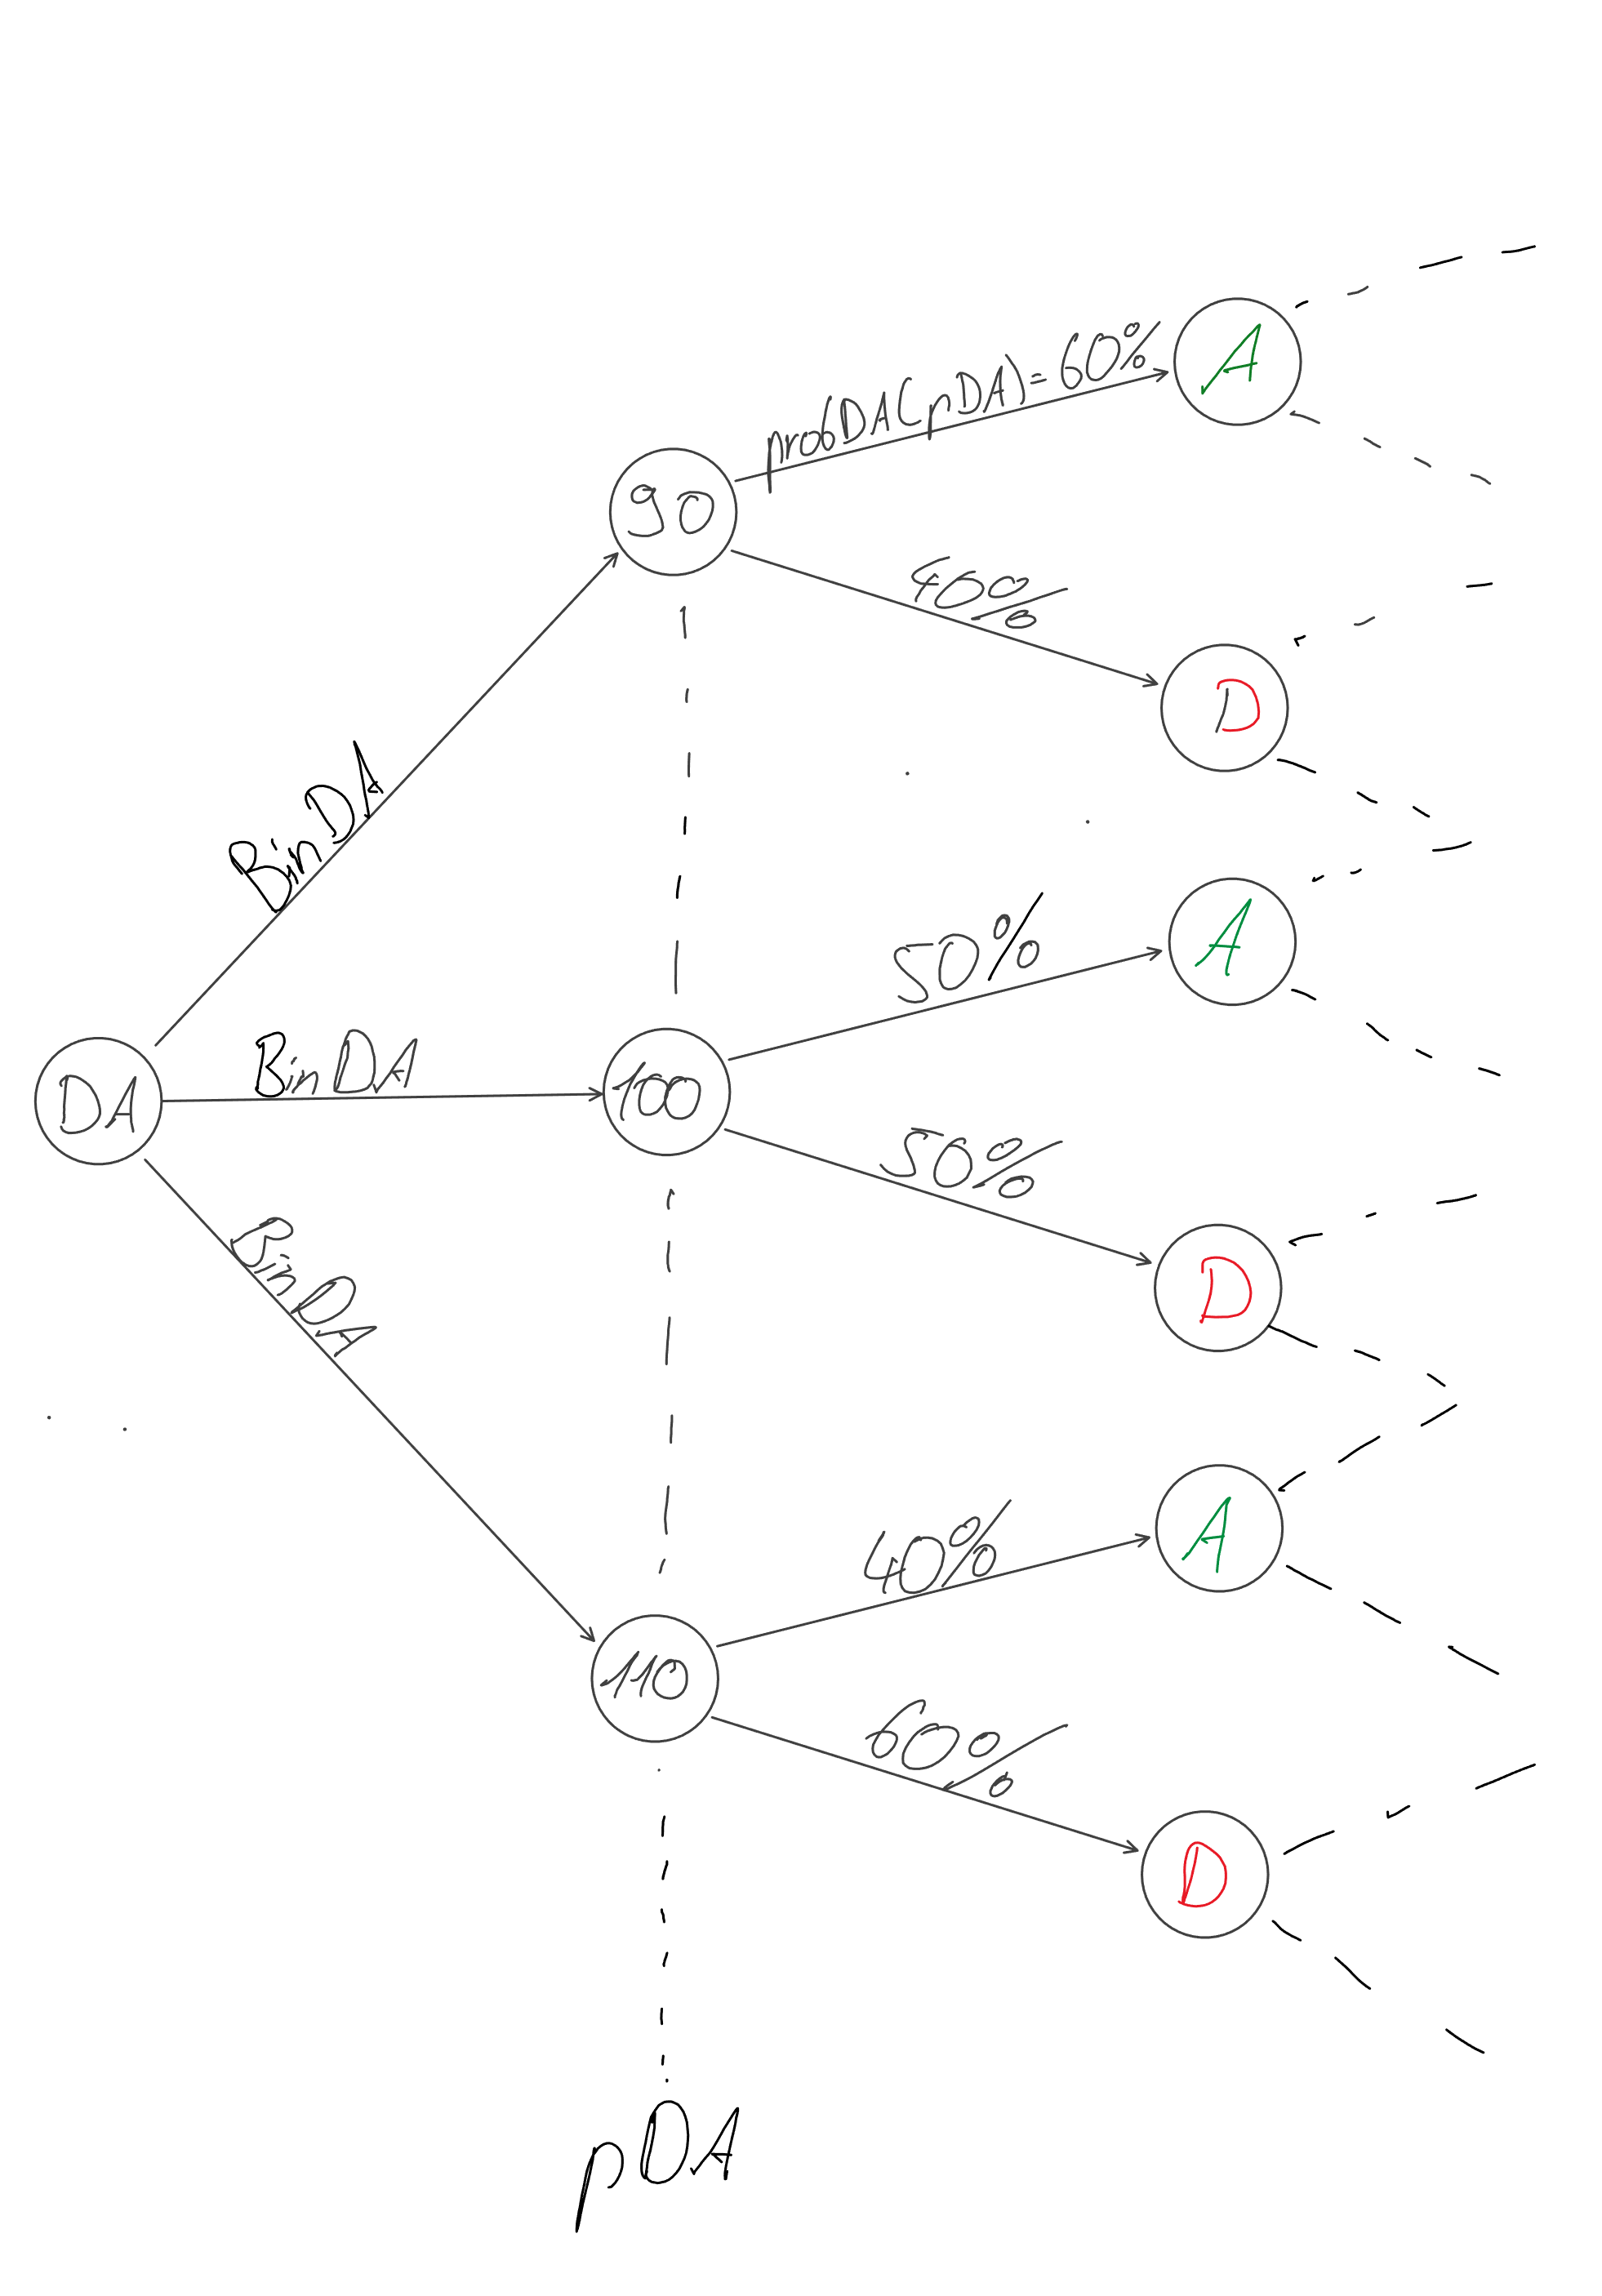
\includegraphics[width=1\linewidth]{pictures/szBaumBeispiel1.png}
    \caption{Beispielhafter Szenariobaum}
    \label{fig:enter-label}
\end{figure}
\todo{grafik neu machen mit tikz und BinDA entfernen}
Zu sehen ist ein Teil des Szenariobaums. Zur Vereinfachung ist in der Abbildung die Mengenentscheidung und die Entscheidung nicht am Day Ahead Markt teil zu nehmen ausgelassen. Zu sehen ist, dass zu verschiedenen Preisen am Day Ahead Markt geboten werden kann. 
Wird eine Entscheidung für einen Preis getroffen fallen entsprechend die anderen Teile des Szenariobaums weg.
Die anschließende Wahrscheinlichkeitsverteilung für ein aktzeptieren des Gebots ist abhängig von der Gebotshöhe aber zufällig.
In der folgenden Abbildung ist beispielhaft die Entscheidung für einen Preis von 90 grün markiert. Die entfallenden anderen Baumabschnitte sind rot markiert.\\

\begin{figure}[H]

    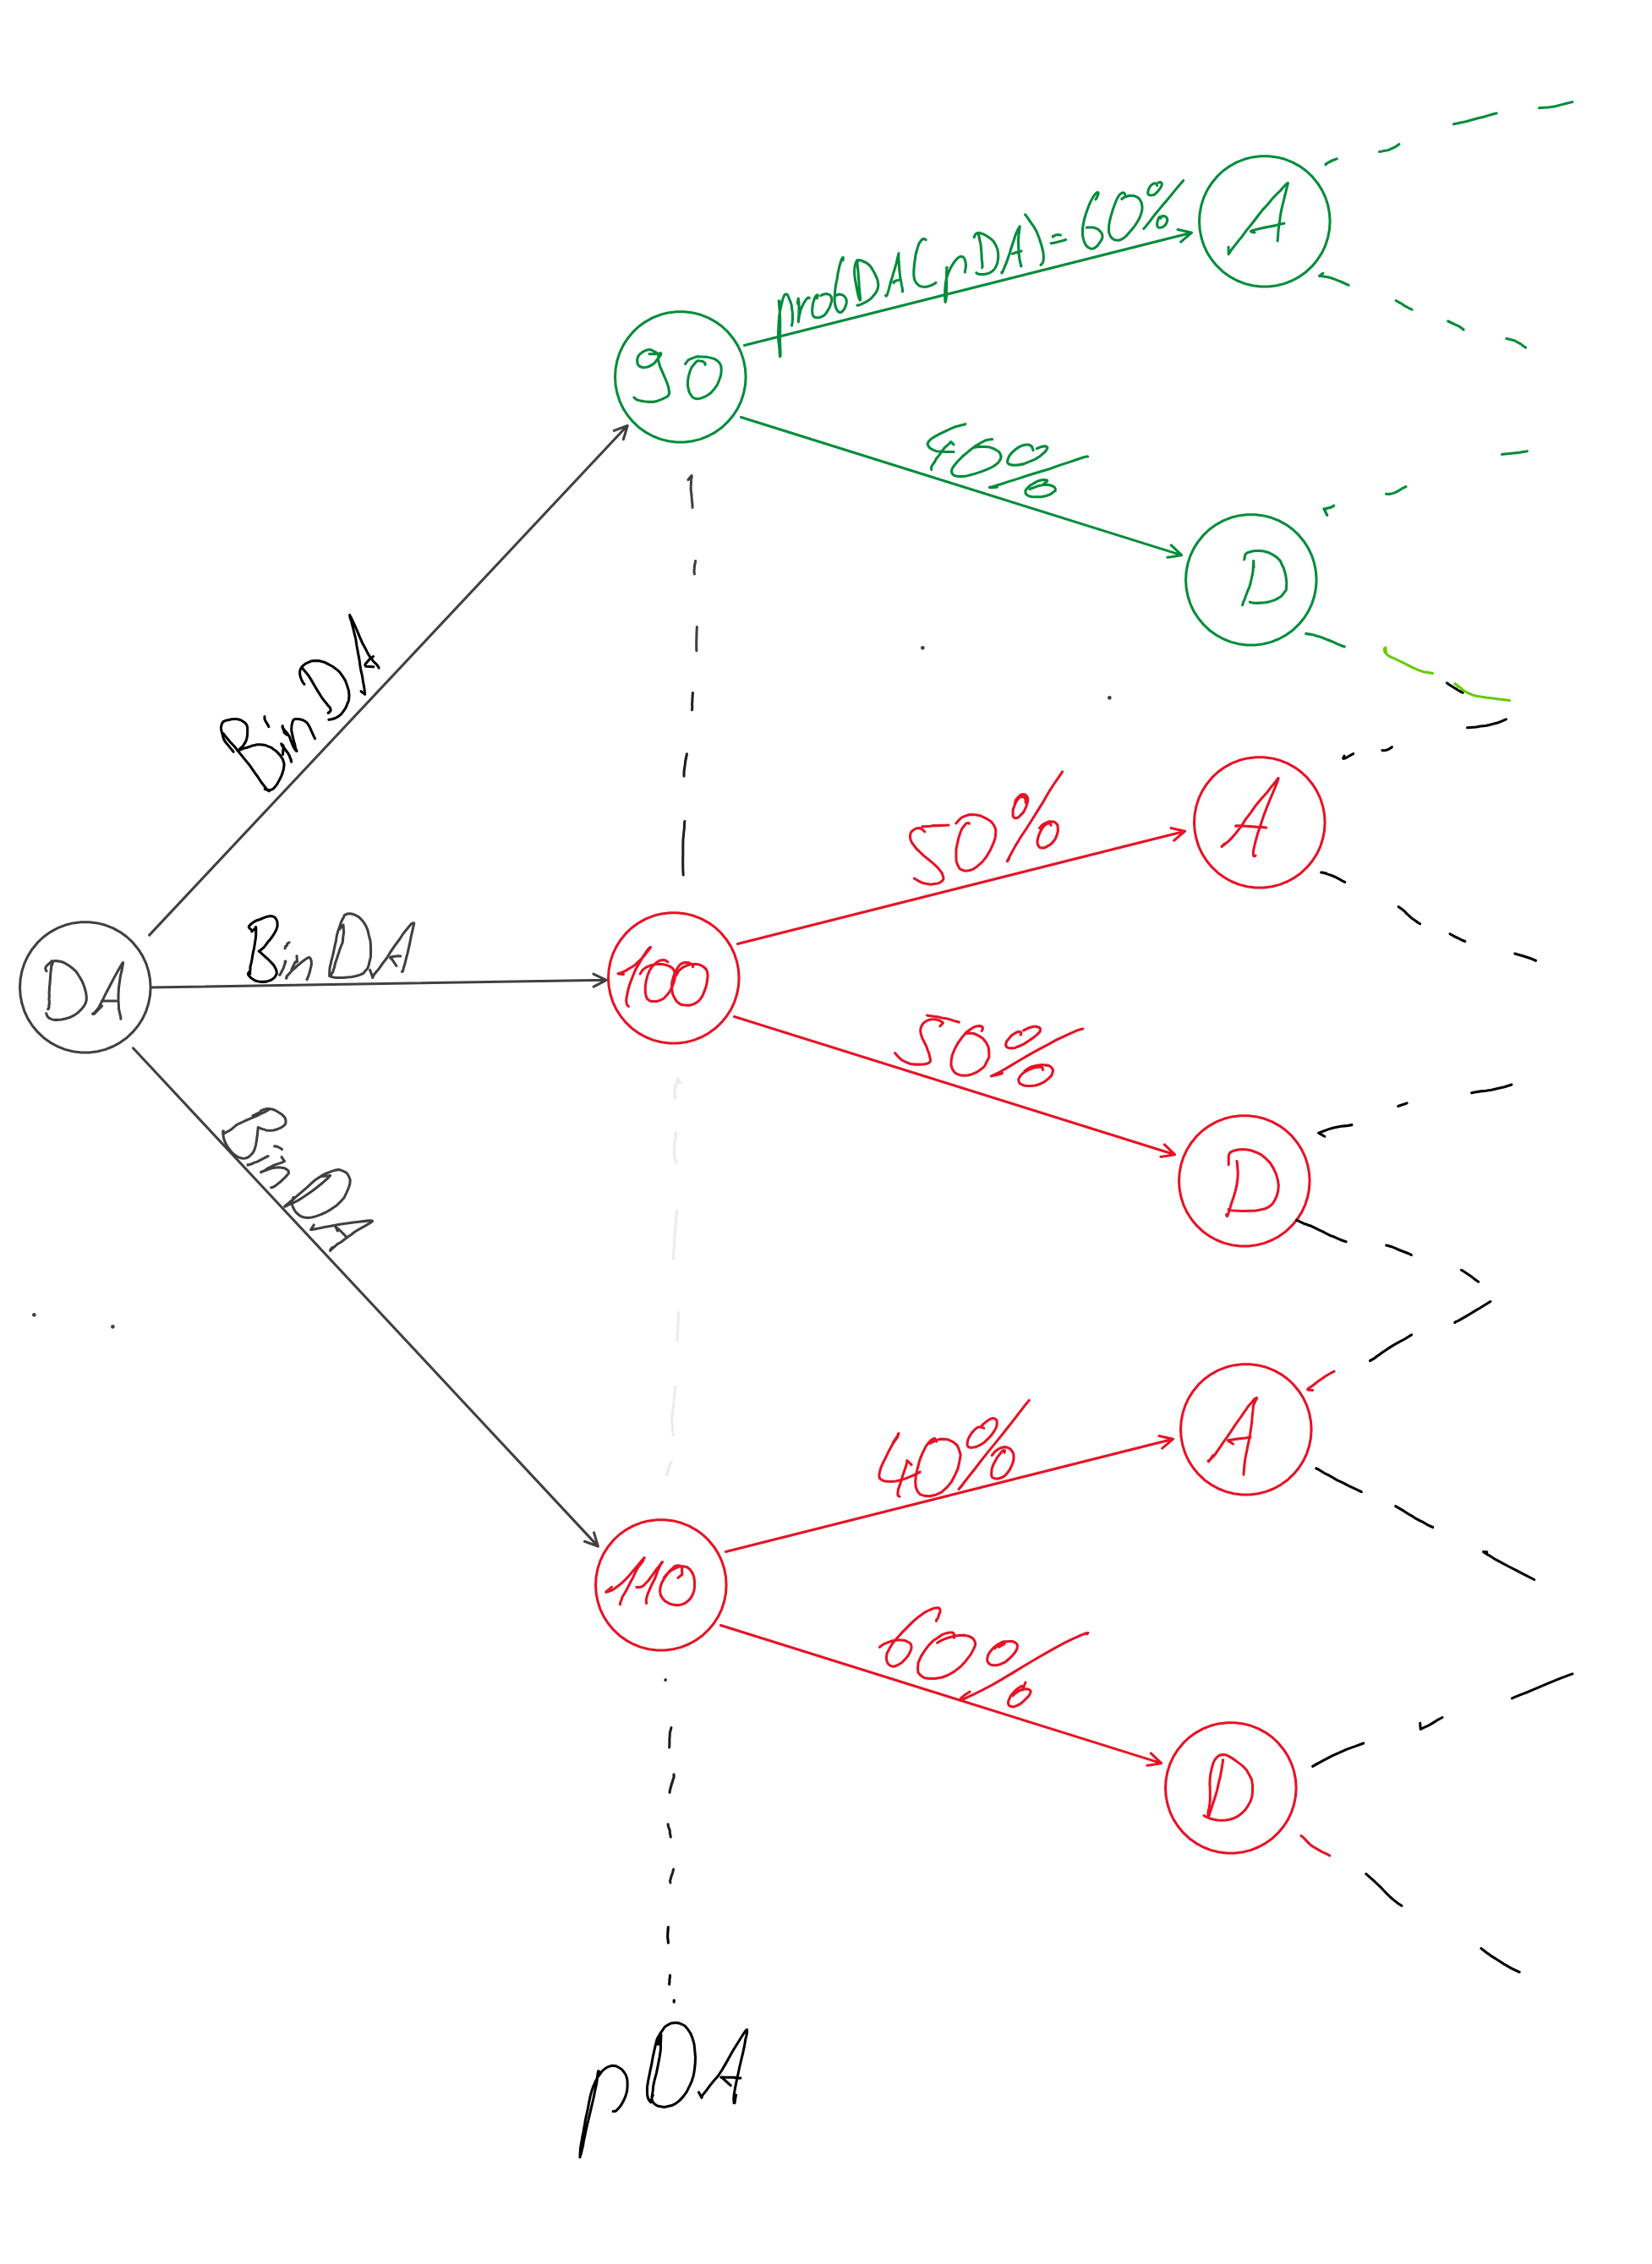
\includegraphics[width=1\linewidth]{pictures/szBaumBeispiel_markiert.png}
    \caption{Beispielhafter Szenariobaum mit markierter Entscheidung}
    \label{fig:enter-label}
\end{figure}
\todo{grafik neu machen mit tikz und BinDA entfernen}

Die Wahrscheinlichkeiten in den aktivierten Teilbäumen addieren sich zu 1 auf.
Anschließend würden sich die folgenden Märkte abbilden (hier mit gestrichelten Linien dargestellt).\\

\subsubsection{Von Umwandlung in lineares Problem}
Bisher erfolgte eine Betrachtung mit dem besonderen Augenmerk auf die Preiswahrscheinlichkeit-Kombination.
Im folgenden wird der Ausdruck $Q_{DA}$ besonders analysiert. Zunächst wird eine weitere binäre Variable eingefügt die signalisiert ob der Abruf der bereitgestellten Leistung wirklich erfolgt.
Hierraus ergibt sich:

    $B^Q_{DA} * Q_{DA}$ 

Da dieser Ausdruck zu einem nicht linearen gemischten ganzzahligen Problem führt ist es sinnvoll dieses in ein lineares Problem umzuwandeln  um die Berechenbarkeit zu verbesseren.
Dies erfolgt über eine Dummy Variable $X_{DA}$. Die Dummy Variable wird anschließend so restriktiert, dass sie sich wie $B^Q_{DA} * Q_{DA}$ verhält.
\\
Nebenbedingungen:\\
$X_{DA} \leq B^Q_{DA} * R$\\
$Q_{DA} - X_{DA} \geq (1 - B^Q_{DA}) * R$\\
$Q_{DA} - X_{DA} \geq 0 $\\
Aus den Nebenbedingung folgt entsprechend:\\
$X_{DA} = B^Q_{DA} * Q_{DA}$\\

So wird aus dem nicht linearen Problem\\
$Ertrag_{DA} = B^Q_{DA} * Q_{DA} * \sum_{s_{DA}}  p_{DA}(s_{DA}) * \omega_{DA}(s_{DA})  $\\
Das lineare Problem\\
$Ertrag_{DA} = X_{DA} * \sum_{s_{DA}} * p_{DA}(s_{DA}) * \omega_{DA}(s_{DA})  $\\
s.t.:\\
$\sum_{s_{DA}} = 1$\\
$X_{DA} \leq B^Q_{DA} * R$\\
$Q_{DA} - X_{DA} \geq (1 - B^Q_{DA}) * R$\\
$Q_{DA} - X_{DA} \geq 0 $\\

\\
\\
\\
$Ertrag_{L} = B^Q_{L} * Q_{L} * \sum_{s_{L}} B^P_{L}(s_{L}) * p_{L}(s_{L}) * \omega_{L}(s_{L})  $\\
\end{document}
